2\centerline{\Huge \bf  Домашнее задание }
\centerline{\Huge \bf Осевая и центральная симметрия}

\begin{flushright}
    \scriptsize{А вы думали я шутки шучу?}
\end{flushright}

\problem{1!}
а) На листе прозрачной бумаги нарисован угол. Как без всяких инструментов построить биссектрису этого угла? После этого покажите, как построить центр вписанной окружности для треугольника, нарисованного на той же прозрачной бумаге.

\noindentб) На листе прозрачной бумаги нарисован отрезок. Как без всяких инструментов построить серединный перпендикуляр к этому отрезку? После этого покажите, как построить центр описанной окружности для треугольника, нарисованного на той же прозрачной бумаге.

\problem{2!} 
а) Известно, что у некоторого многоугольника есть ось симметрии. Сколько вершин может на ней лежать. Для каждого случая приведите пример конкретного многоугольника.

\noindentб) Перечислите все четырёхугольники, имеющие ось симметрии.

\noindentв) По одну сторону от реки Волга находятся населённые пункты Большой Царын и Малые Дербеты. Герман начинает свой путь в Малых Дербетах и направляется в Большой Царын. Герман очень хочет по пути искупаться в реке Волга, при этом пройдя как можно меньшее расстояние. Постройте самый оптимальный путь для Германа.

\begin{wrapfigure}{r}{0.3\linewidth}
    \centering
    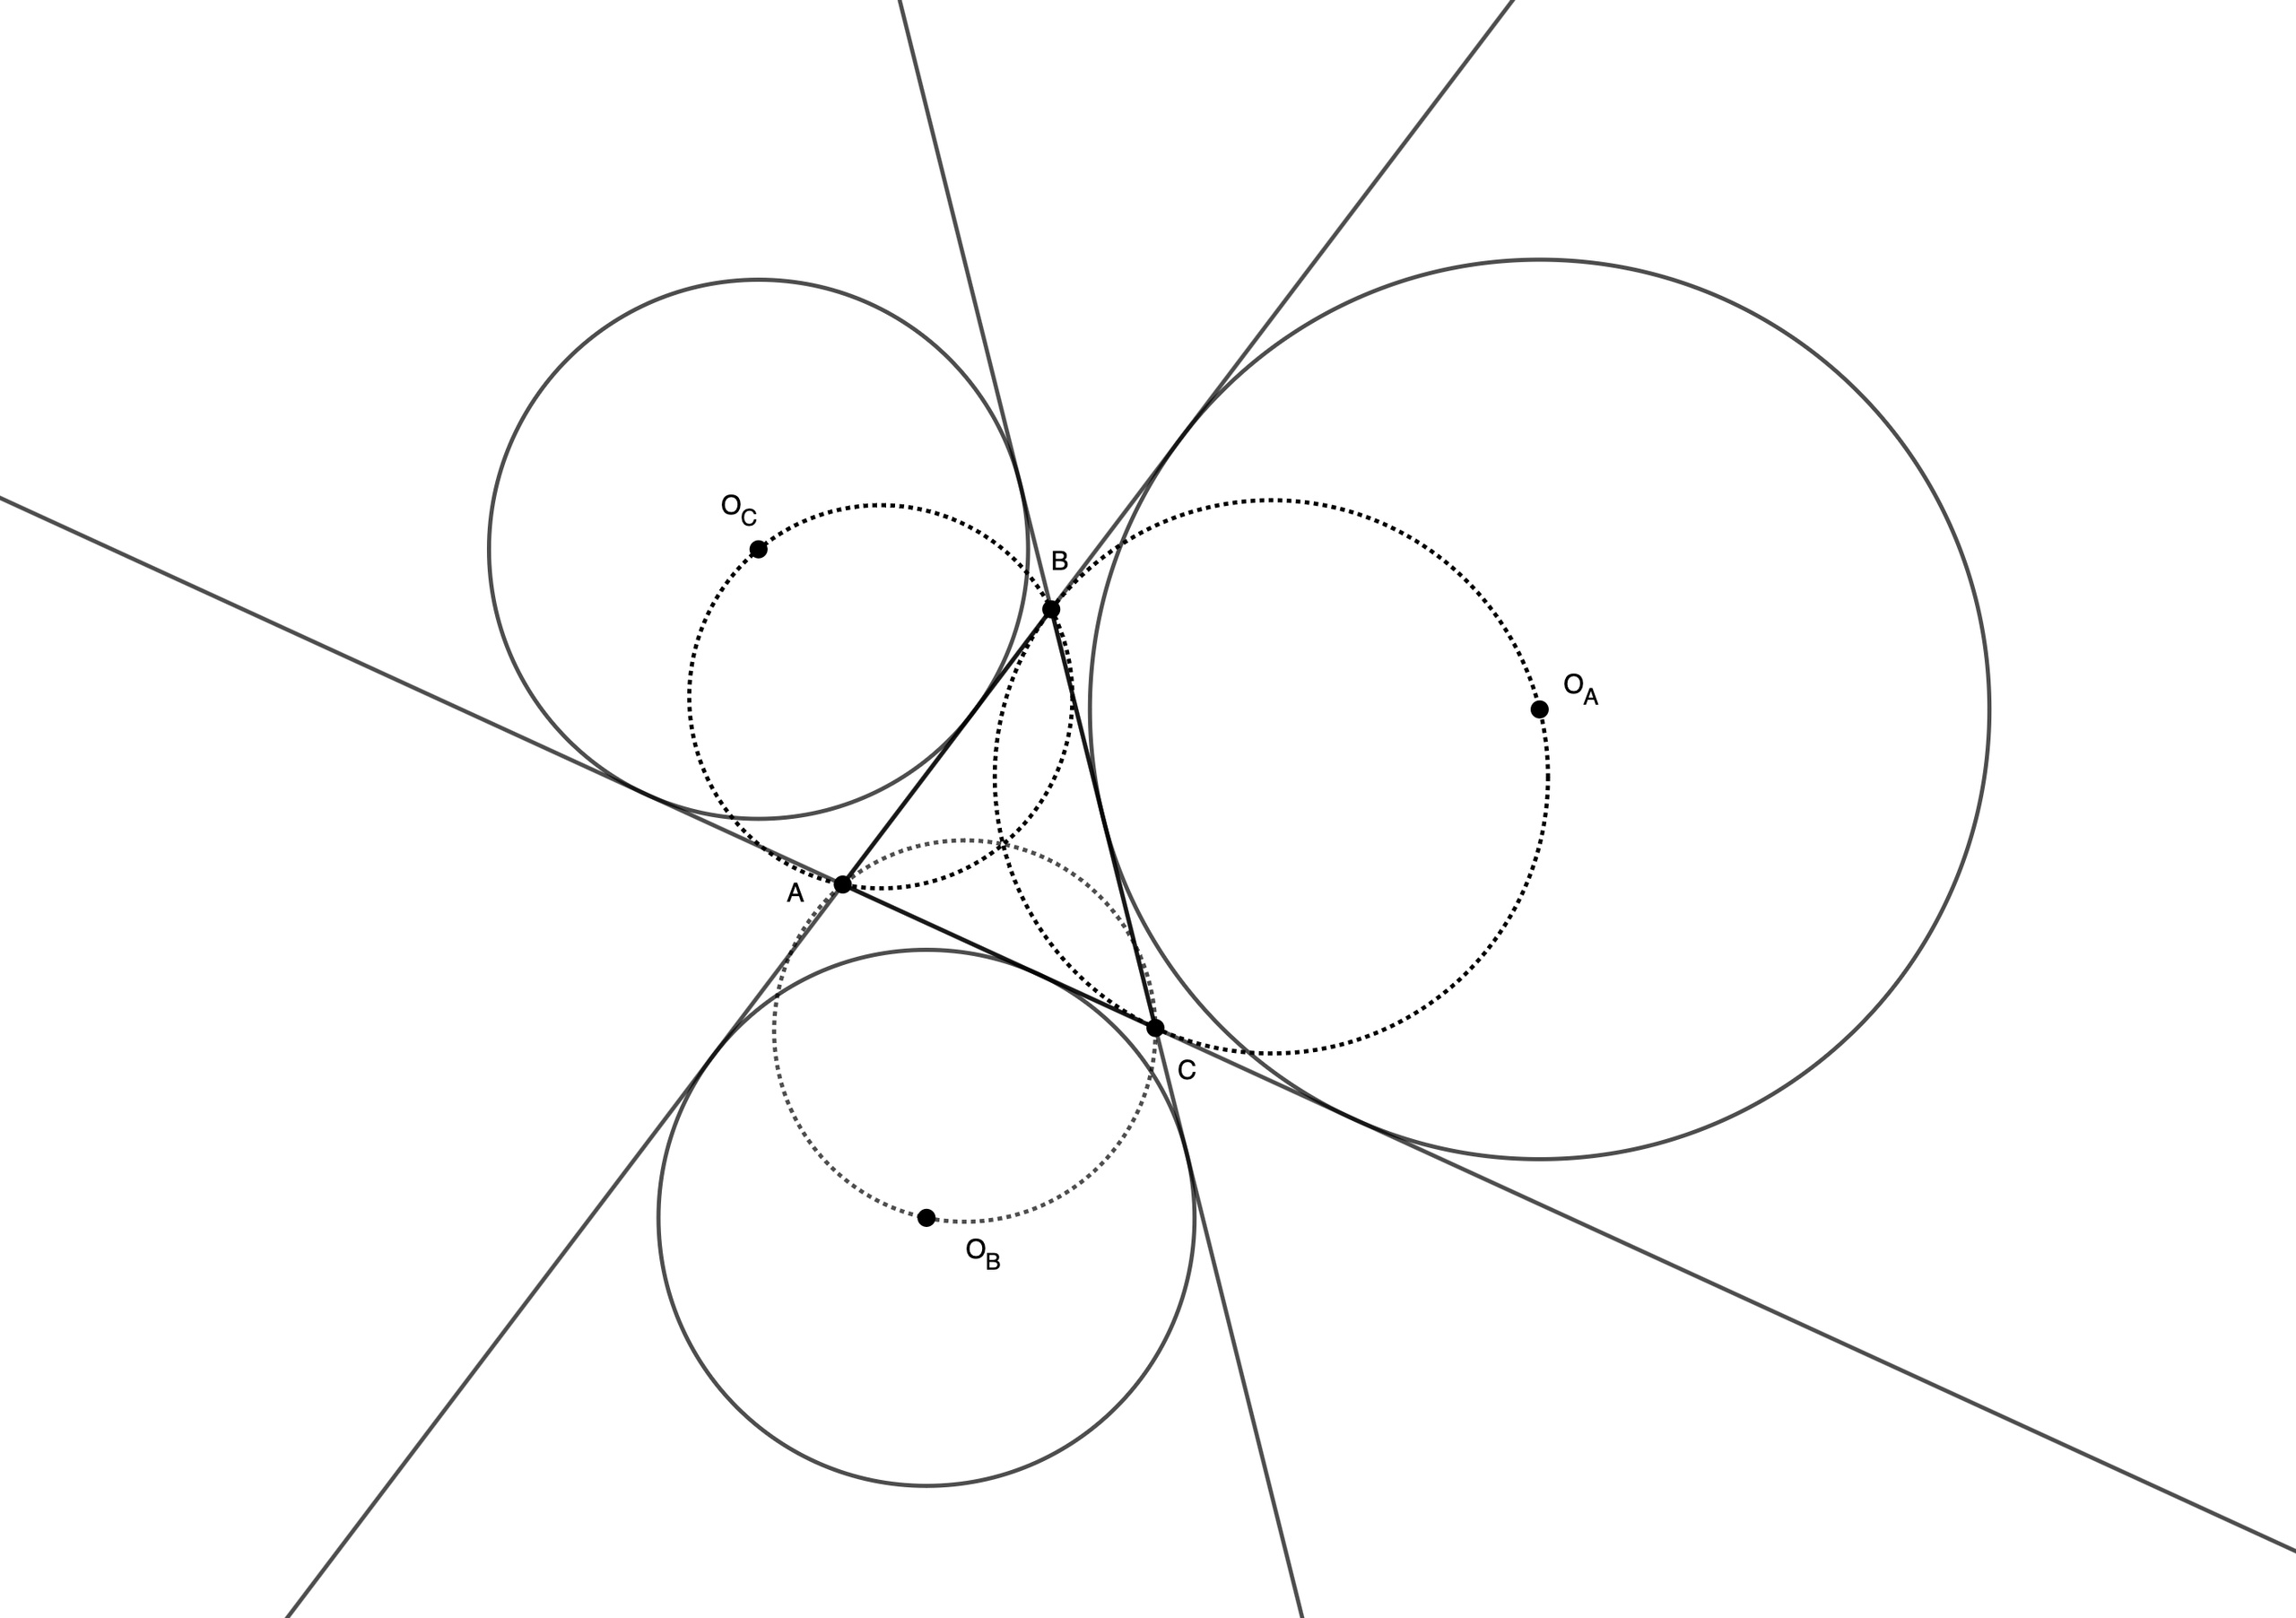
\includegraphics[width=\linewidth]{VII блок/Киви/lesson_2/HW_Simmetry.jpeg}
\end{wrapfigure}

\problem{3} \textit{(Не на симметрию)}
Стороны треугольника $ABC$ продолжены во все стороны. Окружность называется \textit{вневписанной}, если она касается внутренней части одной стороны и продолжения двух других. Для треугольника $ABC$ построены все три вневписанные окружности с центрами в точках $O_{A},\ O_{B},\ O_{C}$ (см. рисунок). Докажите, что окружности, описанные вокруг треугольников $\vartriangle O_{A}BC,\vartriangle O_{B}AC,\vartriangle O_{C}AB$ пересекаются в одной точке.

\problem{4} Бильярдный стол представляет собой бесконечный угол  $AOB$. Внутри него выбраны две лунки (точки) $X$ и $Y$, таким образом, что $\angle AOX = \angle BOY$. Шар вылетел из лунки $X$ ударился о стенку $OA$ и упруго(угол падения равен углу отражения) отскочил прямо в лунку $Y$. После этого он вылетел из лунки $Y$, отскочил от стенки $OB$ и упруго отскочил прямо в лунку $X$. Докажите, что длина траектории из $X$ в $Y$ равна длине траектории из $Y$ в $X$.
